%%%%%%%%%%%%%%%%%%%%%%%%%%%%%%%%%%%%%%%%%%%%%%%%%%%%%%%%%%%%%%%%%%%
% Header: General study / work / project template
%%%%%%%%%%%%%%%%%%%%%%%%%%%%%%%%%%%%%%%%%%%%%%%%%%%%%%%%%%%%%%%%%%%

\documentclass[11pt,a4paper]{scrartcl}

% Layout
\usepackage[margin=2.5cm]{geometry}
\usepackage{setspace}
\setstretch{1.15}

% General packages
\usepackage{graphicx}
\usepackage{enumitem}
\usepackage[most]{tcolorbox}
\tcbuselibrary{breakable}
\usepackage[breaklinks=true,colorlinks=true,linkcolor=blue,urlcolor=blue,citecolor=blue]{hyperref}
\usepackage{amsmath,amsthm,amssymb,mathtools}
\usepackage{braket}
\usepackage{icomma}
\usepackage[T1]{fontenc}
\usepackage[utf8]{inputenc}
\usepackage[ngerman]{babel}

% Units / tables / floats / references
\usepackage[locale = DE,space-before-unit=true,per-mode = symbol]{siunitx}
\usepackage{booktabs,multirow}
\usepackage{placeins}
\usepackage[natbib,abbreviate=true,doi=false,style=numeric-comp,giveninits=true,sorting=none]{biblatex}
\usepackage{csquotes}

% Optional math shortcuts
\newcommand{\R}{\mathbb{R}}
\newcommand{\N}{\mathbb{N}}
\newcommand{\Q}{\mathbb{Q}}
\newcommand{\abs}[1]{\left| #1 \right|}
\newcommand{\norm}[1]{\left\lVert #1 \right\rVert}
\newcommand{\ol}[1]{\overline{#1}}
\newcommand{\op}[1]{\hat{#1}}
\newcommand{\e}{\mathrm e}
\newcommand{\ii}{\mathrm i}
\newcommand{\eps}{\varepsilon}

% Box styles
\newtcolorbox{calculationbox}[1][]{
    title=Calculation,
    breakable,
    enhanced,
    colback=white,
    colframe=black!65,
    #1
}

\newtcolorbox{solutionbox}[1][]{
    title=Solution,
    breakable,
    enhanced,
    colback=white,
    colframe=black!65,
    #1
}

\newtcolorbox{answerbox}[1][]{
    title=Answer,
    breakable,
    enhanced,
    colback=white,
    colframe=black!65,
    #1
}

\newtcolorbox{notebox}[1][]{
    title=Notes,
    breakable,
    enhanced,
    colback=white,
    colframe=black!65,
    #1
}

\newtcolorbox{sidecalcbox}[1][]{
    title=Side Calculation,
    breakable,
    enhanced,
    colback=white,
    colframe=black!65,
    #1
}

%%%%%%%%%%%%%%%%%%%%%%%%%%%%%%%%%%%%%%%%%%%%%%%%%%%%%%%%%%%%%%%%%%%
\begin{document}

    \title{Theoretische Physik 2 -- Blatt 11}
    \author{Tobias Laser}
    \date{\today}
    \maketitle
    \vfill
    \thispagestyle{empty}
    \newpage

    \pagenumbering{arabic}

    % ================================================================
    \paragraph{26. Aufgabe 1: Bloch-Vektor}

    In der Vorlesung wurde gezeigt, dass jeder normierte Qubit-Zustand als Punkt auf der Einheitskugel dargestellt werden kann. Ein Qubit befinde sich im Zustand
    \begin{align*}
        \ket{\psi}
        =
        \cos\left(\frac{\theta}{2}\right)\ket{0}
        +
        \e^{\ii\varphi}\sin\left(\frac{\theta}{2}\right)\ket{1}.
    \end{align*}

    \begin{enumerate}[label=(\alph*)]
        \item Zeigen Sie, dass der Zustand dem folgenden Bloch-Vektor entspricht:
        \begin{align*}
            \vec n=
            \left(
                \sin\theta\cos\varphi,
                \sin\theta\sin\varphi,
                \cos\theta
            \right).
        \end{align*}

        \begin{calculationbox}
            Die Idee ist, dass ein reiner Qubit-Zustand durch die Erwartungswerte der Pauli-Matrizen beschrieben werden kann:
            \begin{align*}
                \vec n
                =
                \left(
                    \braket{\sigma_x},
                    \braket{\sigma_y},
                    \braket{\sigma_z}
                \right),
                \qquad
                \braket{\sigma_i}
                =
                \bra{\psi}\sigma_i\ket{\psi}.
            \end{align*}
            Wir berechnen diese drei Erwartungswerte explizit.

            \begin{calculationbox}[title=Darstellung des Zustands als Spaltenvektor]
                In der Basis
                \begin{align*}
                    \ket{0}=
                    \begin{pmatrix}
                        1\\0
                    \end{pmatrix},
                    \qquad
                    \ket{1}=
                    \begin{pmatrix}
                        0\\1
                    \end{pmatrix}
                \end{align*}
                schreiben wir
                \begin{align*}
                    \ket{\psi}
                    =
                    \begin{pmatrix}
                        \cos\left(\frac{\theta}{2}\right)\\[0.3em]
                        \e^{\ii\varphi}\sin\left(\frac{\theta}{2}\right)
                    \end{pmatrix}.
                \end{align*}
                Zur Abkürzung setzen wir
                \begin{align*}
                    c=\cos\left(\frac{\theta}{2}\right),
                    \qquad
                    s=\sin\left(\frac{\theta}{2}\right).
                \end{align*}
                Dann gilt
                \begin{align*}
                    \ket{\psi}
                    =
                    \begin{pmatrix}
                        c\\
                        \e^{\ii\varphi}s
                    \end{pmatrix},
                    \qquad
                    \bra{\psi}
                    =
                    \begin{pmatrix}
                        c & \e^{-\ii\varphi}s
                    \end{pmatrix}.
                \end{align*}
            \end{calculationbox}

            \begin{calculationbox}[title=Erwartungswert von $\sigma_x$]
                Die Pauli-Matrix $\sigma_x$ ist
                \begin{align*}
                    \sigma_x=
                    \begin{pmatrix}
                        0&1\\
                        1&0
                    \end{pmatrix}.
                \end{align*}
                Daher
                \begin{align*}
                    \sigma_x\ket{\psi}
                    =
                    \begin{pmatrix}
                        \e^{\ii\varphi}s\\
                        c
                    \end{pmatrix}.
                \end{align*}
                Damit folgt
                \begin{align*}
                    \braket{\sigma_x}
                    &=
                    \bra{\psi}\sigma_x\ket{\psi}\\
                    &=
                    \begin{pmatrix}
                        c & \e^{-\ii\varphi}s
                    \end{pmatrix}
                    \begin{pmatrix}
                        \e^{\ii\varphi}s\\
                        c
                    \end{pmatrix}\\
                    &=
                    cs\e^{\ii\varphi}
                    +
                    cs\e^{-\ii\varphi}\\
                    &=
                    cs\left(\e^{\ii\varphi}+\e^{-\ii\varphi}\right)\\
                    &=
                    2cs\cos\varphi.
                \end{align*}
                Mit
                \begin{align*}
                    2\sin\left(\frac{\theta}{2}\right)\cos\left(\frac{\theta}{2}\right)
                    =
                    \sin\theta
                \end{align*}
                ergibt sich
                \begin{align*}
                    \braket{\sigma_x}
                    =
                    \sin\theta\cos\varphi.
                \end{align*}
            \end{calculationbox}

            \begin{calculationbox}[title=Erwartungswert von $\sigma_y$]
                Die Pauli-Matrix $\sigma_y$ ist
                \begin{align*}
                    \sigma_y=
                    \begin{pmatrix}
                        0&-\ii\\
                        \ii&0
                    \end{pmatrix}.
                \end{align*}
                Daher
                \begin{align*}
                    \sigma_y\ket{\psi}
                    =
                    \begin{pmatrix}
                        -\ii\e^{\ii\varphi}s\\
                        \ii c
                    \end{pmatrix}.
                \end{align*}
                Damit folgt
                \begin{align*}
                    \braket{\sigma_y}
                    &=
                    \bra{\psi}\sigma_y\ket{\psi}\\
                    &=
                    \begin{pmatrix}
                        c & \e^{-\ii\varphi}s
                    \end{pmatrix}
                    \begin{pmatrix}
                        -\ii\e^{\ii\varphi}s\\
                        \ii c
                    \end{pmatrix}\\
                    &=
                    -\ii cs\e^{\ii\varphi}
                    +
                    \ii cs\e^{-\ii\varphi}\\
                    &=
                    \ii cs\left(\e^{-\ii\varphi}-\e^{\ii\varphi}\right).
                \end{align*}
                Wegen
                \begin{align*}
                    \e^{\ii\varphi}-\e^{-\ii\varphi}=2\ii\sin\varphi
                \end{align*}
                erhalten wir
                \begin{align*}
                    \braket{\sigma_y}
                    =
                    2cs\sin\varphi
                    =
                    \sin\theta\sin\varphi.
                \end{align*}
            \end{calculationbox}

            \begin{calculationbox}[title=Erwartungswert von $\sigma_z$]
                Die Pauli-Matrix $\sigma_z$ ist
                \begin{align*}
                    \sigma_z=
                    \begin{pmatrix}
                        1&0\\
                        0&-1
                    \end{pmatrix}.
                \end{align*}
                Daher
                \begin{align*}
                    \sigma_z\ket{\psi}
                    =
                    \begin{pmatrix}
                        c\\
                        -\e^{\ii\varphi}s
                    \end{pmatrix}.
                \end{align*}
                Damit folgt
                \begin{align*}
                    \braket{\sigma_z}
                    &=
                    \bra{\psi}\sigma_z\ket{\psi}\\
                    &=
                    \begin{pmatrix}
                        c & \e^{-\ii\varphi}s
                    \end{pmatrix}
                    \begin{pmatrix}
                        c\\
                        -\e^{\ii\varphi}s
                    \end{pmatrix}\\
                    &=
                    c^2-s^2\\
                    &=
                    \cos^2\left(\frac{\theta}{2}\right)
                    -
                    \sin^2\left(\frac{\theta}{2}\right)\\
                    &=
                    \cos\theta.
                \end{align*}
            \end{calculationbox}

            \begin{solutionbox}[title=Bloch-Vektor]
                Die drei Komponenten des Bloch-Vektors sind
                \begin{align*}
                    n_x&=\braket{\sigma_x}=\sin\theta\cos\varphi,\\
                    n_y&=\braket{\sigma_y}=\sin\theta\sin\varphi,\\
                    n_z&=\braket{\sigma_z}=\cos\theta.
                \end{align*}
                Also entspricht der Zustand
                \begin{align*}
                    \ket{\psi}
                    =
                    \cos\left(\frac{\theta}{2}\right)\ket{0}
                    +
                    \e^{\ii\varphi}\sin\left(\frac{\theta}{2}\right)\ket{1}
                \end{align*}
                dem Bloch-Vektor
                \begin{align*}
                    \vec n=
                    \left(
                        \sin\theta\cos\varphi,
                        \sin\theta\sin\varphi,
                        \cos\theta
                    \right).
                \end{align*}
            \end{solutionbox}
        \end{calculationbox}

        \item Skizzieren Sie diesen Zustand auf der Bloch-Sphäre für $\theta=\pi/2$ und $\varphi=\pi/2$. Skizzieren Sie weiterhin die Zustände
        \begin{align*}
            \frac{\ket{0}+\ket{1}}{\sqrt2},
            \qquad
            \frac{\ket{0}-\ii\ket{1}}{\sqrt2}
        \end{align*}
        auf der Bloch-Kugel.

        \begin{calculationbox}
            Wir verwenden die Zuordnung
            \begin{align*}
                \vec n=
                \left(
                    \sin\theta\cos\varphi,
                    \sin\theta\sin\varphi,
                    \cos\theta
                \right).
            \end{align*}
            Damit kann man jeden der drei Zustände als Punkt auf der Einheitskugel eintragen.

            \begin{calculationbox}[title={Zustand mit $\theta=\pi/2$ und $\varphi=\pi/2$}]
                Einsetzen ergibt
                \begin{align*}
                    \vec n
                    &=
                    \left(
                        \sin\left(\frac{\pi}{2}\right)\cos\left(\frac{\pi}{2}\right),
                        \sin\left(\frac{\pi}{2}\right)\sin\left(\frac{\pi}{2}\right),
                        \cos\left(\frac{\pi}{2}\right)
                    \right)\\
                    &=
                    (0,1,0).
                \end{align*}
                Dieser Zustand liegt also auf der positiven $y$-Achse.
                Der zugehörige Zustand ist
                \begin{align*}
                    \ket{\psi}
                    =
                    \frac{1}{\sqrt2}\ket{0}
                    +
                    \frac{\ii}{\sqrt2}\ket{1}
                    =
                    \frac{\ket{0}+\ii\ket{1}}{\sqrt2}.
                \end{align*}
            \end{calculationbox}

            \begin{calculationbox}[title=Zustand $(\ket{0}+\ket{1})/\sqrt2$]
                Wir vergleichen mit
                \begin{align*}
                    \ket{\psi}
                    =
                    \cos\left(\frac{\theta}{2}\right)\ket{0}
                    +
                    \e^{\ii\varphi}\sin\left(\frac{\theta}{2}\right)\ket{1}.
                \end{align*}
                Aus
                \begin{align*}
                    \frac{\ket{0}+\ket{1}}{\sqrt2}
                \end{align*}
                folgt
                \begin{align*}
                    \cos\left(\frac{\theta}{2}\right)=\frac1{\sqrt2},
                    \qquad
                    \sin\left(\frac{\theta}{2}\right)=\frac1{\sqrt2},
                    \qquad
                    \e^{\ii\varphi}=1.
                \end{align*}
                Also ist
                \begin{align*}
                    \theta=\frac{\pi}{2},
                    \qquad
                    \varphi=0.
                \end{align*}
                Damit
                \begin{align*}
                    \vec n
                    =
                    (1,0,0).
                \end{align*}
                Dieser Zustand liegt auf der positiven $x$-Achse.
            \end{calculationbox}

            \begin{calculationbox}[title=Zustand $(\ket{0}-\ii\ket{1})/\sqrt2$]
                Hier gilt
                \begin{align*}
                    \frac{\ket{0}-\ii\ket{1}}{\sqrt2}.
                \end{align*}
                Wieder ist
                \begin{align*}
                    \theta=\frac{\pi}{2}.
                \end{align*}
                Außerdem ist der relative Phasenfaktor
                \begin{align*}
                    \e^{\ii\varphi}=-\ii
                    =
                    \e^{-\ii\pi/2}.
                \end{align*}
                Also ist
                \begin{align*}
                    \varphi=-\frac{\pi}{2}
                    \qquad
                    \text{oder äquivalent}
                    \qquad
                    \varphi=\frac{3\pi}{2}.
                \end{align*}
                Damit
                \begin{align*}
                    \vec n
                    &=
                    \left(
                        \sin\left(\frac{\pi}{2}\right)\cos\left(-\frac{\pi}{2}\right),
                        \sin\left(\frac{\pi}{2}\right)\sin\left(-\frac{\pi}{2}\right),
                        \cos\left(\frac{\pi}{2}\right)
                    \right)\\
                    &=
                    (0,-1,0).
                \end{align*}
                Dieser Zustand liegt auf der negativen $y$-Achse.
            \end{calculationbox}

            \begin{solutionbox}[title=Skizze auf der Bloch-Sphäre]
                Die drei Punkte auf der Bloch-Sphäre sind
                \begin{align*}
                    \theta=\frac{\pi}{2},\ \varphi=\frac{\pi}{2}
                    &\quad\Longrightarrow\quad
                    \vec n=(0,1,0),
                    \\[0.3em]
                    \frac{\ket{0}+\ket{1}}{\sqrt2}
                    &\quad\Longrightarrow\quad
                    \vec n=(1,0,0),
                    \\[0.3em]
                    \frac{\ket{0}-\ii\ket{1}}{\sqrt2}
                    &\quad\Longrightarrow\quad
                    \vec n=(0,-1,0).
                \end{align*}
                Für die Skizze zeichnet man die Einheitskugel mit $x$-, $y$- und $z$-Achse. Die drei Zustände liegen alle auf dem Äquator:
                \begin{align*}
                    (1,0,0)\text{ auf }+x,
                    \qquad
                    (0,1,0)\text{ auf }+y,
                    \qquad
                    (0,-1,0)\text{ auf }-y.
                \end{align*}
            \end{solutionbox}
        \end{calculationbox}

        \item Betrachten Sie nun den Hamiltonoperator
        \begin{align*}
            H(\omega,\Omega)
            =
            \hbar\omega\sigma_z+\hbar\Omega\sigma_x.
        \end{align*}
        Zeigen Sie, dass
        \begin{align*}
            U_x(t)=\exp\left[-\frac{\ii}{\hbar}H(0,\Omega)t\right],
            \qquad
            U_z(t)=\exp\left[-\frac{\ii}{\hbar}H(\omega,0)t\right]
        \end{align*}
        Drehungen auf der Bloch-Sphäre um die $x$- und $z$-Achse entsprechen. Zeigen Sie dies durch explizite Anwendung der Zeitentwicklungsoperatoren auf den Zustand $\ket{\psi}$.

        \begin{calculationbox}
            Wir betrachten zuerst die beiden Spezialfälle getrennt. Für
            \begin{align*}
                H(0,\Omega)=\hbar\Omega\sigma_x
            \end{align*}
            ist die Zeitentwicklung durch $\sigma_x$ erzeugt. Für
            \begin{align*}
                H(\omega,0)=\hbar\omega\sigma_z
            \end{align*}
            ist die Zeitentwicklung durch $\sigma_z$ erzeugt.

            \begin{calculationbox}[title=Exponentialformel für Pauli-Matrizen]
                Für jede Pauli-Matrix gilt
                \begin{align*}
                    \sigma_i^2=\mathbb{1}.
                \end{align*}
                Deshalb kann man die Exponentialreihe in gerade und ungerade Potenzen aufteilen:
                \begin{align*}
                    \e^{-\ii a\sigma_i}
                    &=
                    \sum_{n=0}^{\infty}\frac{(-\ii a\sigma_i)^n}{n!}\\
                    &=
                    \mathbb{1}
                    \sum_{k=0}^{\infty}
                    \frac{(-1)^k a^{2k}}{(2k)!}
                    -
                    \ii\sigma_i
                    \sum_{k=0}^{\infty}
                    \frac{(-1)^k a^{2k+1}}{(2k+1)!}\\
                    &=
                    \mathbb{1}\cos a-\ii\sigma_i\sin a.
                \end{align*}
                Also gilt
                \begin{align*}
                    \e^{-\ii a\sigma_i}
                    =
                    \cos a\,\mathbb{1}
                    -
                    \ii\sin a\,\sigma_i.
                \end{align*}
            \end{calculationbox}

            \begin{calculationbox}[title=Zeitentwicklung um die $z$-Achse]
                Für
                \begin{align*}
                    H(\omega,0)=\hbar\omega\sigma_z
                \end{align*}
                gilt
                \begin{align*}
                    U_z(t)
                    =
                    \exp(-\ii\omega t\sigma_z).
                \end{align*}
                Da
                \begin{align*}
                    \sigma_z\ket{0}=+\ket{0},
                    \qquad
                    \sigma_z\ket{1}=-\ket{1},
                \end{align*}
                folgt
                \begin{align*}
                    U_z(t)\ket{0}
                    =
                    \e^{-\ii\omega t}\ket{0},
                    \qquad
                    U_z(t)\ket{1}
                    =
                    \e^{+\ii\omega t}\ket{1}.
                \end{align*}
                Anwenden auf den allgemeinen Zustand liefert
                \begin{align*}
                    U_z(t)\ket{\psi}
                    &=
                    \cos\left(\frac{\theta}{2}\right)
                    \e^{-\ii\omega t}\ket{0}
                    +
                    \e^{\ii\varphi}
                    \sin\left(\frac{\theta}{2}\right)
                    \e^{+\ii\omega t}\ket{1}\\
                    &=
                    \e^{-\ii\omega t}
                    \left[
                        \cos\left(\frac{\theta}{2}\right)\ket{0}
                        +
                        \e^{\ii(\varphi+2\omega t)}
                        \sin\left(\frac{\theta}{2}\right)\ket{1}
                    \right].
                \end{align*}
                Der Faktor $\e^{-\ii\omega t}$ ist eine globale Phase und hat keinen Einfluss auf den Bloch-Vektor. Also ändert sich nur
                \begin{align*}
                    \varphi\mapsto \varphi+2\omega t,
                    \qquad
                    \theta\mapsto\theta.
                \end{align*}
                Damit wird
                \begin{align*}
                    \vec n
                    =
                    \left(
                        \sin\theta\cos\varphi,
                        \sin\theta\sin\varphi,
                        \cos\theta
                    \right)
                \end{align*}
                zu
                \begin{align*}
                    \vec n\,'
                    =
                    \left(
                        \sin\theta\cos(\varphi+2\omega t),
                        \sin\theta\sin(\varphi+2\omega t),
                        \cos\theta
                    \right).
                \end{align*}
                Das ist eine Drehung um die $z$-Achse mit Winkel $2\omega t$.
            \end{calculationbox}

            \begin{calculationbox}[title=Zeitentwicklung um die $x$-Achse]
                Für
                \begin{align*}
                    H(0,\Omega)=\hbar\Omega\sigma_x
                \end{align*}
                gilt
                \begin{align*}
                    U_x(t)
                    =
                    \exp(-\ii\Omega t\sigma_x)
                    =
                    \cos(\Omega t)\mathbb{1}
                    -
                    \ii\sin(\Omega t)\sigma_x.
                \end{align*}
                Mit
                \begin{align*}
                    \sigma_x\ket{0}=\ket{1},
                    \qquad
                    \sigma_x\ket{1}=\ket{0}
                \end{align*}
                folgt
                \begin{align*}
                    U_x(t)\ket{0}
                    &=
                    \cos(\Omega t)\ket{0}
                    -
                    \ii\sin(\Omega t)\ket{1},
                    \\
                    U_x(t)\ket{1}
                    &=
                    \cos(\Omega t)\ket{1}
                    -
                    \ii\sin(\Omega t)\ket{0}.
                \end{align*}
                Wir setzen wieder
                \begin{align*}
                    c=\cos\left(\frac{\theta}{2}\right),
                    \qquad
                    s=\sin\left(\frac{\theta}{2}\right),
                    \qquad
                    a=\Omega t.
                \end{align*}
                Dann ist
                \begin{align*}
                    \ket{\psi}
                    =
                    c\ket{0}
                    +
                    \e^{\ii\varphi}s\ket{1}.
                \end{align*}
                Also
                \begin{align*}
                    U_x(t)\ket{\psi}
                    &=
                    c\left(\cos a\ket{0}-\ii\sin a\ket{1}\right)
                    +
                    \e^{\ii\varphi}s
                    \left(\cos a\ket{1}-\ii\sin a\ket{0}\right)\\
                    &=
                    \left(c\cos a-\ii\e^{\ii\varphi}s\sin a\right)\ket{0}
                    +
                    \left(\e^{\ii\varphi}s\cos a-\ii c\sin a\right)\ket{1}.
                \end{align*}
                Dies ist wieder ein normierter Qubit-Zustand. Um die Wirkung auf der Bloch-Sphäre zu sehen, berechnen wir die neuen Erwartungswerte. Man erhält nach Einsetzen in
                \begin{align*}
                    n_x'=2\mathrm{Re}(\alpha'^*\beta'),
                    \qquad
                    n_y'=2\mathrm{Im}(\alpha'^*\beta'),
                    \qquad
                    n_z'=|\alpha'|^2-|\beta'|^2
                \end{align*}
                die Transformation
                \begin{align*}
                    n_x'&=n_x,\\
                    n_y'&=n_y\cos(2\Omega t)-n_z\sin(2\Omega t),\\
                    n_z'&=n_y\sin(2\Omega t)+n_z\cos(2\Omega t).
                \end{align*}
                Die $x$-Komponente bleibt also fest, während die $y$- und $z$-Komponenten ineinander rotieren. Das ist genau eine Drehung um die $x$-Achse mit Winkel $2\Omega t$.
            \end{calculationbox}

            \begin{solutionbox}[title=Drehungen auf der Bloch-Sphäre]
                Die Zeitentwicklung durch
                \begin{align*}
                    H(0,\Omega)=\hbar\Omega\sigma_x
                \end{align*}
                entspricht einer Drehung des Bloch-Vektors um die $x$-Achse:
                \begin{align*}
                    \vec n\,'
                    =
                    \begin{pmatrix}
                        1&0&0\\
                        0&\cos(2\Omega t)&-\sin(2\Omega t)\\
                        0&\sin(2\Omega t)&\cos(2\Omega t)
                    \end{pmatrix}
                    \vec n.
                \end{align*}
                Die Zeitentwicklung durch
                \begin{align*}
                    H(\omega,0)=\hbar\omega\sigma_z
                \end{align*}
                entspricht einer Drehung des Bloch-Vektors um die $z$-Achse:
                \begin{align*}
                    \vec n\,'
                    =
                    \begin{pmatrix}
                        \cos(2\omega t)&-\sin(2\omega t)&0\\
                        \sin(2\omega t)&\cos(2\omega t)&0\\
                        0&0&1
                    \end{pmatrix}
                    \vec n.
                \end{align*}
                Der Faktor $2$ entsteht, weil der Zeitentwicklungsoperator die Form $\exp(-\ii a\sigma_i)$ hat, während die zugehörige räumliche Drehung auf der Bloch-Sphäre den Winkel $2a$ besitzt.
            \end{solutionbox}
        \end{calculationbox}

        \item Bonus: Gehen Sie zurück zu Aufgabe 17(c) aus Übungsblatt 7, Magnetische Resonanz und Rabiformel. Skizzieren Sie die Dynamik des Zustands auf der Bloch-Kugel im mitrotierenden System.

        \begin{calculationbox}
            Im mitrotierenden System wird die explizite Zeitabhängigkeit des Hamiltonoperators entfernt. Für die Koeffizienten
            \begin{align*}
                b_+(t)=\e^{+\ii\omega t/2}a_+(t),
                \qquad
                b_-(t)=\e^{-\ii\omega t/2}a_-(t)
            \end{align*}
            ergibt sich die Gleichung
            \begin{align*}
                \ii\frac{d}{dt}
                \begin{pmatrix}
                    b_+\\
                    b_-
                \end{pmatrix}
                =
                \begin{pmatrix}
                    -\Delta\omega/2 & \omega_1/2\\
                    \omega_1/2 & +\Delta\omega/2
                \end{pmatrix}
                \begin{pmatrix}
                    b_+\\
                    b_-
                \end{pmatrix},
            \end{align*}
            wobei
            \begin{align*}
                \Delta\omega=\omega-\omega_0
            \end{align*}
            die Verstimmung ist.

            \begin{calculationbox}[title=Effektiver Hamiltonoperator]
                Die Matrix kann mit Pauli-Matrizen geschrieben werden als
                \begin{align*}
                    H_{\mathrm{rot}}
                    =
                    \frac{\hbar}{2}
                    \left(
                        \omega_1\sigma_x
                        -
                        \Delta\omega\,\sigma_z
                    \right).
                \end{align*}
                Der effektive Feldvektor im mitrotierenden System ist also proportional zu
                \begin{align*}
                    \vec \Omega_{\mathrm{eff}}
                    =
                    \left(
                        \omega_1,
                        0,
                        -\Delta\omega
                    \right).
                \end{align*}
                Seine Länge ist
                \begin{align*}
                    \Omega_R
                    =
                    \sqrt{\omega_1^2+\Delta\omega^2}.
                \end{align*}
                Diese Frequenz ist die verallgemeinerte Rabi-Frequenz.
            \end{calculationbox}

            \begin{calculationbox}[title=Bewegung des Bloch-Vektors]
                Auf der Bloch-Kugel bedeutet der Hamiltonoperator
                \begin{align*}
                    H_{\mathrm{rot}}
                    =
                    \frac{\hbar}{2}\vec\Omega_{\mathrm{eff}}\cdot\vec\sigma
                \end{align*}
                eine Präzession des Bloch-Vektors um die Achse $\vec\Omega_{\mathrm{eff}}$.

                Wird der Spin anfangs in
                \begin{align*}
                    \ket{\psi(0)}=\ket{+}
                \end{align*}
                präpariert, dann startet der Bloch-Vektor am Nordpol:
                \begin{align*}
                    \vec n(0)=(0,0,1).
                \end{align*}
                Im mitrotierenden System rotiert dieser Vektor mit Frequenz
                \begin{align*}
                    \Omega_R=\sqrt{\omega_1^2+\Delta\omega^2}
                \end{align*}
                um die Achse
                \begin{align*}
                    \vec\Omega_{\mathrm{eff}}
                    =
                    (\omega_1,0,-\Delta\omega).
                \end{align*}
            \end{calculationbox}

            \begin{calculationbox}[title=Resonanz und Nichtresonanz]
                Auf Resonanz gilt
                \begin{align*}
                    \Delta\omega=0.
                \end{align*}
                Dann liegt die effektive Drehachse entlang der $x$-Achse:
                \begin{align*}
                    \vec\Omega_{\mathrm{eff}}=(\omega_1,0,0).
                \end{align*}
                Der Bloch-Vektor rotiert dann vom Nordpol zum Südpol und wieder zurück. Deshalb kann die Übergangswahrscheinlichkeit bis auf $1$ anwachsen:
                \begin{align*}
                    P_-(t)=\sin^2\left(\frac{\omega_1t}{2}\right).
                \end{align*}

                Außerhalb der Resonanz gilt
                \begin{align*}
                    \Delta\omega\neq 0.
                \end{align*}
                Dann ist die Drehachse gegen die $z$-Achse geneigt. Der Bloch-Vektor kreist um diese schiefe Achse und erreicht im Allgemeinen nicht mehr den Südpol. Die maximale Übergangswahrscheinlichkeit ist dann kleiner als $1$:
                \begin{align*}
                    P_-(t)
                    =
                    \frac{\omega_1^2}{\omega_1^2+\Delta\omega^2}
                    \sin^2\left(
                        \frac{\sqrt{\omega_1^2+\Delta\omega^2}}{2}t
                    \right).
                \end{align*}
            \end{calculationbox}

            \begin{solutionbox}[title=Skizze der Rabi-Dynamik auf der Bloch-Kugel]
                Im mitrotierenden System führt der Bloch-Vektor eine Präzession um die effektive Achse
                \begin{align*}
                    \vec\Omega_{\mathrm{eff}}
                    =
                    (\omega_1,0,-\Delta\omega)
                \end{align*}
                aus. Für die Skizze:
                \begin{itemize}
                    \item Bei $\Delta\omega=0$ zeichnet man eine Drehachse entlang $x$. Der Zustand läuft auf einem Großkreis vom Nordpol zum Südpol.
                    \item Bei $\Delta\omega\neq0$ zeichnet man eine schiefe Drehachse in der $xz$-Ebene. Der Zustand läuft auf einem Kreis um diese Achse und erreicht den Südpol im Allgemeinen nicht.
                \end{itemize}
                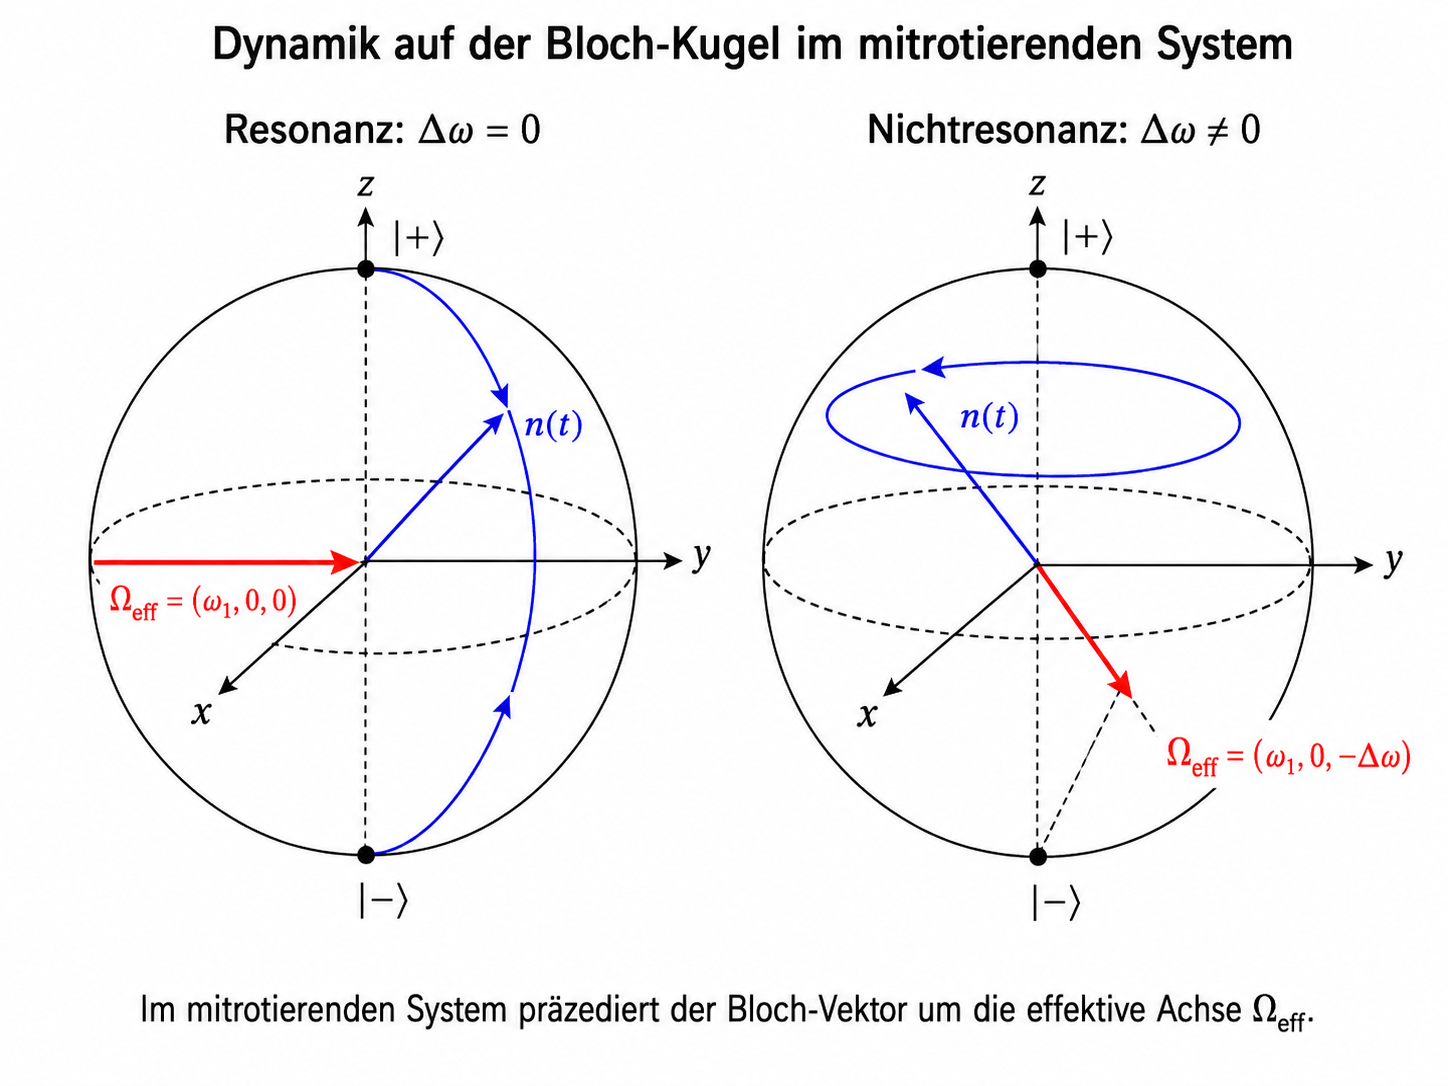
\includegraphics[width=0.9\textwidth]{178fd4f9-1761-4ff6-a4fd-d1165ff4998b.png}
            \end{solutionbox}
        \end{calculationbox}
    \end{enumerate}

    % ================================================================
    \paragraph{27. Aufgabe 2: Verschränkung zweier Qubits}

    Betrachten Sie den Zustand
    \begin{align*}
        \ket{\Phi^+}
        =
        \frac{\ket{00}+\ket{11}}{\sqrt2}.
    \end{align*}

    \begin{enumerate}[label=(\alph*)]
        \item Zeigen Sie, dass der Zustand normiert ist.

        \begin{calculationbox}
            Ein Zustand ist normiert, wenn sein Skalarprodukt mit sich selbst gleich $1$ ist:
            \begin{align*}
                \braket{\Phi^+|\Phi^+}=1.
            \end{align*}

            \begin{calculationbox}[title=Normierung]
                Wir verwenden die Orthonormalität der Zweiqubit-Basis:
                \begin{align*}
                    \braket{00|00}=1,
                    \qquad
                    \braket{11|11}=1,
                    \qquad
                    \braket{00|11}=0,
                    \qquad
                    \braket{11|00}=0.
                \end{align*}
                Dann gilt
                \begin{align*}
                    \braket{\Phi^+|\Phi^+}
                    &=
                    \frac{1}{2}
                    \left(
                        \bra{00}+\bra{11}
                    \right)
                    \left(
                        \ket{00}+\ket{11}
                    \right)\\
                    &=
                    \frac{1}{2}
                    \left(
                        \braket{00|00}
                        +
                        \braket{00|11}
                        +
                        \braket{11|00}
                        +
                        \braket{11|11}
                    \right)\\
                    &=
                    \frac{1}{2}(1+0+0+1)\\
                    &=
                    1.
                \end{align*}
            \end{calculationbox}

            \begin{solutionbox}[title=Normierung]
                Der Bell-Zustand
                \begin{align*}
                    \ket{\Phi^+}
                    =
                    \frac{\ket{00}+\ket{11}}{\sqrt2}
                \end{align*}
                ist normiert, weil
                \begin{align*}
                    \braket{\Phi^+|\Phi^+}=1.
                \end{align*}
            \end{solutionbox}
        \end{calculationbox}

        \item Zeigen Sie, dass sich der Zustand nicht in der Form
        \begin{align*}
            \ket{\Phi^+}
            =
            (a\ket{0}+b\ket{1})\otimes(c\ket{0}+d\ket{1})
        \end{align*}
        schreiben lässt. Der Zustand ist also nicht separabel und daher verschränkt.

        \begin{calculationbox}
            Ein Zweiqubit-Zustand ist separabel, wenn er als Produkt zweier Einqubit-Zustände geschrieben werden kann. Wir nehmen an, dass das möglich ist, und zeigen dann einen Widerspruch.

            \begin{calculationbox}[title=Allgemeiner separabler Zustand]
                Wir multiplizieren den allgemeinen Produktzustand aus:
                \begin{align*}
                    (a\ket{0}+b\ket{1})\otimes(c\ket{0}+d\ket{1})
                    &=
                    ac\ket{00}
                    +
                    ad\ket{01}
                    +
                    bc\ket{10}
                    +
                    bd\ket{11}.
                \end{align*}
                Damit dieser Zustand gleich
                \begin{align*}
                    \ket{\Phi^+}
                    =
                    \frac{1}{\sqrt2}\ket{00}
                    +
                    0\ket{01}
                    +
                    0\ket{10}
                    +
                    \frac{1}{\sqrt2}\ket{11}
                \end{align*}
                ist, müssten die Koeffizienten erfüllen:
                \begin{align*}
                    ac=\frac1{\sqrt2},
                    \qquad
                    ad=0,
                    \qquad
                    bc=0,
                    \qquad
                    bd=\frac1{\sqrt2}.
                \end{align*}
            \end{calculationbox}

            \begin{calculationbox}[title=Widerspruch]
                Aus
                \begin{align*}
                    ac=\frac1{\sqrt2}
                \end{align*}
                folgt insbesondere
                \begin{align*}
                    a\neq0,
                    \qquad
                    c\neq0.
                \end{align*}
                Aus
                \begin{align*}
                    ad=0
                \end{align*}
                und $a\neq0$ folgt
                \begin{align*}
                    d=0.
                \end{align*}
                Aus
                \begin{align*}
                    bc=0
                \end{align*}
                und $c\neq0$ folgt
                \begin{align*}
                    b=0.
                \end{align*}
                Dann ist aber
                \begin{align*}
                    bd=0.
                \end{align*}
                Das widerspricht der notwendigen Bedingung
                \begin{align*}
                    bd=\frac1{\sqrt2}.
                \end{align*}
            \end{calculationbox}

            \begin{solutionbox}[title=Nicht-Separabilität]
                Der Zustand
                \begin{align*}
                    \ket{\Phi^+}
                    =
                    \frac{\ket{00}+\ket{11}}{\sqrt2}
                \end{align*}
                kann nicht als Produkt zweier Einqubit-Zustände geschrieben werden. Daher ist er nicht separabel. Also ist $\ket{\Phi^+}$ ein verschränkter Zustand.
            \end{solutionbox}
        \end{calculationbox}

        \item Alice und Bob teilen sich den Bell-Zustand $\ket{\Phi^+}$. Alice bekommt das erste Qubit und Bob das zweite. Alice misst ihr Qubit in der Rechenbasis $\{\ket{0},\ket{1}\}$. Mit welchen Wahrscheinlichkeiten erhält Alice die Ergebnisse $0$ bzw. $1$?

        \begin{calculationbox}
            Der Zustand ist
            \begin{align*}
                \ket{\Phi^+}
                =
                \frac{\ket{00}+\ket{11}}{\sqrt2}.
            \end{align*}
            Das erste Qubit gehört Alice. Wir lesen deshalb die Wahrscheinlichkeiten aus den Anteilen mit erstem Qubit $\ket{0}$ beziehungsweise $\ket{1}$ ab.

            \begin{calculationbox}[title=Messwahrscheinlichkeit für Alice]
                Der Anteil mit Alice-Zustand $\ket{0}$ ist
                \begin{align*}
                    \frac{1}{\sqrt2}\ket{00}.
                \end{align*}
                Also ist
                \begin{align*}
                    P_A(0)
                    =
                    \abs{\frac1{\sqrt2}}^2
                    =
                    \frac12.
                \end{align*}
                Der Anteil mit Alice-Zustand $\ket{1}$ ist
                \begin{align*}
                    \frac{1}{\sqrt2}\ket{11}.
                \end{align*}
                Also ist
                \begin{align*}
                    P_A(1)
                    =
                    \abs{\frac1{\sqrt2}}^2
                    =
                    \frac12.
                \end{align*}
            \end{calculationbox}

            \begin{solutionbox}[title=Messwahrscheinlichkeiten von Alice]
                Alice erhält
                \begin{align*}
                    P_A(0)=\frac12,
                    \qquad
                    P_A(1)=\frac12.
                \end{align*}
                Beide Messergebnisse sind also gleich wahrscheinlich.
            \end{solutionbox}
        \end{calculationbox}

        \item Welcher Zustand bleibt für Bob jeweils übrig, falls Alice das Ergebnis $0$ bzw. $1$ erhält?

        \begin{calculationbox}
            Bei einer Messung wird der Zustand auf den Anteil projiziert, der zum gemessenen Ergebnis passt. Danach muss der Zustand wieder normiert werden.

            \begin{calculationbox}[title=Alice misst $0$]
                Wenn Alice das Ergebnis $0$ misst, bleibt aus
                \begin{align*}
                    \ket{\Phi^+}
                    =
                    \frac{\ket{00}+\ket{11}}{\sqrt2}
                \end{align*}
                nur der Anteil mit erstem Qubit $\ket{0}$ übrig:
                \begin{align*}
                    \frac1{\sqrt2}\ket{00}.
                \end{align*}
                Nach Normierung ist der Gesamtzustand
                \begin{align*}
                    \ket{00}.
                \end{align*}
                Daher ist Bobs Zustand
                \begin{align*}
                    \ket{0}.
                \end{align*}
            \end{calculationbox}

            \begin{calculationbox}[title=Alice misst $1$]
                Wenn Alice das Ergebnis $1$ misst, bleibt nur der Anteil mit erstem Qubit $\ket{1}$ übrig:
                \begin{align*}
                    \frac1{\sqrt2}\ket{11}.
                \end{align*}
                Nach Normierung ist der Gesamtzustand
                \begin{align*}
                    \ket{11}.
                \end{align*}
                Daher ist Bobs Zustand
                \begin{align*}
                    \ket{1}.
                \end{align*}
            \end{calculationbox}

            \begin{solutionbox}[title=Zustand von Bob nach Alices Messung]
                Für den Zustand
                \begin{align*}
                    \ket{\Phi^+}
                    =
                    \frac{\ket{00}+\ket{11}}{\sqrt2}
                \end{align*}
                gilt:
                \begin{align*}
                    \text{Alice misst }0
                    &\quad\Longrightarrow\quad
                    \text{Bob hat }\ket{0},
                    \\
                    \text{Alice misst }1
                    &\quad\Longrightarrow\quad
                    \text{Bob hat }\ket{1}.
                \end{align*}
            \end{solutionbox}
        \end{calculationbox}

        \item Erläutern Sie kurz, weshalb die Messergebnisse von Alice und Bob perfekt korreliert sind.

        \begin{calculationbox}
            Der Zustand
            \begin{align*}
                \ket{\Phi^+}
                =
                \frac{\ket{00}+\ket{11}}{\sqrt2}
            \end{align*}
            enthält nur die beiden Komponenten $\ket{00}$ und $\ket{11}$. Es gibt keine Komponenten $\ket{01}$ oder $\ket{10}$.

            \begin{calculationbox}[title=Korrelation]
                Die möglichen Messergebnisse in der Rechenbasis sind daher nur:
                \begin{align*}
                    00
                    \qquad
                    \text{oder}
                    \qquad
                    11.
                \end{align*}
                Wenn Alice also $0$ misst, muss Bob ebenfalls $0$ messen. Wenn Alice $1$ misst, muss Bob ebenfalls $1$ messen:
                \begin{align*}
                    P(B=0|A=0)=1,
                    \qquad
                    P(B=1|A=1)=1.
                \end{align*}
                Die anders korrelierten Ergebnisse sind unmöglich:
                \begin{align*}
                    P(B=1|A=0)=0,
                    \qquad
                    P(B=0|A=1)=0.
                \end{align*}
            \end{calculationbox}

            \begin{solutionbox}[title=Perfekte Korrelation]
                Alice und Bob sind perfekt korreliert, weil der Bell-Zustand $\ket{\Phi^+}$ nur gleiche Bitwerte enthält:
                \begin{align*}
                    \ket{\Phi^+}
                    =
                    \frac{\ket{00}+\ket{11}}{\sqrt2}.
                \end{align*}
                Bei Messung in der Rechenbasis gilt daher immer
                \begin{align*}
                    A=B.
                \end{align*}
            \end{solutionbox}
        \end{calculationbox}

        \item Wie ändern sich die Ergebnisse in (c)--(e), wenn Alice und Bob stattdessen den Zustand
        \begin{align*}
            \ket{\Psi^+}
            =
            \frac{\ket{01}+\ket{10}}{\sqrt2}
        \end{align*}
        erhalten?

        \begin{calculationbox}
            Der neue Bell-Zustand ist
            \begin{align*}
                \ket{\Psi^+}
                =
                \frac{\ket{01}+\ket{10}}{\sqrt2}.
            \end{align*}
            Wieder gehört das erste Qubit Alice und das zweite Qubit Bob.

            \begin{calculationbox}[title=Messwahrscheinlichkeiten von Alice]
                Der Anteil mit Alice-Zustand $\ket{0}$ ist
                \begin{align*}
                    \frac1{\sqrt2}\ket{01}.
                \end{align*}
                Also
                \begin{align*}
                    P_A(0)
                    =
                    \frac12.
                \end{align*}
                Der Anteil mit Alice-Zustand $\ket{1}$ ist
                \begin{align*}
                    \frac1{\sqrt2}\ket{10}.
                \end{align*}
                Also
                \begin{align*}
                    P_A(1)
                    =
                    \frac12.
                \end{align*}
                Die Einzelwahrscheinlichkeiten von Alice bleiben also unverändert.
            \end{calculationbox}

            \begin{calculationbox}[title=Zustand von Bob nach Alices Messung]
                Wenn Alice $0$ misst, bleibt
                \begin{align*}
                    \ket{01}
                \end{align*}
                übrig. Bob hat dann
                \begin{align*}
                    \ket{1}.
                \end{align*}
                Wenn Alice $1$ misst, bleibt
                \begin{align*}
                    \ket{10}
                \end{align*}
                übrig. Bob hat dann
                \begin{align*}
                    \ket{0}.
                \end{align*}
            \end{calculationbox}

            \begin{calculationbox}[title=Korrelation]
                Im Zustand $\ket{\Psi^+}$ treten nur die Kombinationen
                \begin{align*}
                    01
                    \qquad
                    \text{und}
                    \qquad
                    10
                \end{align*}
                auf. Alice und Bob erhalten also immer verschiedene Ergebnisse:
                \begin{align*}
                    P(B=1|A=0)=1,
                    \qquad
                    P(B=0|A=1)=1.
                \end{align*}
                Die gleichen Ergebnisse treten nicht auf:
                \begin{align*}
                    P(B=0|A=0)=0,
                    \qquad
                    P(B=1|A=1)=0.
                \end{align*}
            \end{calculationbox}

            \begin{solutionbox}[title=Ergebnisse für $\ket{\Psi^+}$]
                Für
                \begin{align*}
                    \ket{\Psi^+}
                    =
                    \frac{\ket{01}+\ket{10}}{\sqrt2}
                \end{align*}
                bleiben Alices Wahrscheinlichkeiten gleich:
                \begin{align*}
                    P_A(0)=\frac12,
                    \qquad
                    P_A(1)=\frac12.
                \end{align*}
                Aber Bobs Zustand ist jeweils der entgegengesetzte:
                \begin{align*}
                    \text{Alice misst }0
                    &\quad\Longrightarrow\quad
                    \text{Bob hat }\ket{1},
                    \\
                    \text{Alice misst }1
                    &\quad\Longrightarrow\quad
                    \text{Bob hat }\ket{0}.
                \end{align*}
                Die Messergebnisse sind also nicht gleich korreliert, sondern perfekt antikorreliert:
                \begin{align*}
                    A\neq B.
                \end{align*}
            \end{solutionbox}
        \end{calculationbox}
    \end{enumerate}

\end{document}
```
